\section{mail\-Account Class Reference}
\label{classmailAccount}\index{mailAccount@{mailAccount}}
mail plugin  


Inheritance diagram for mail\-Account::\begin{figure}[H]
\begin{center}
\leavevmode
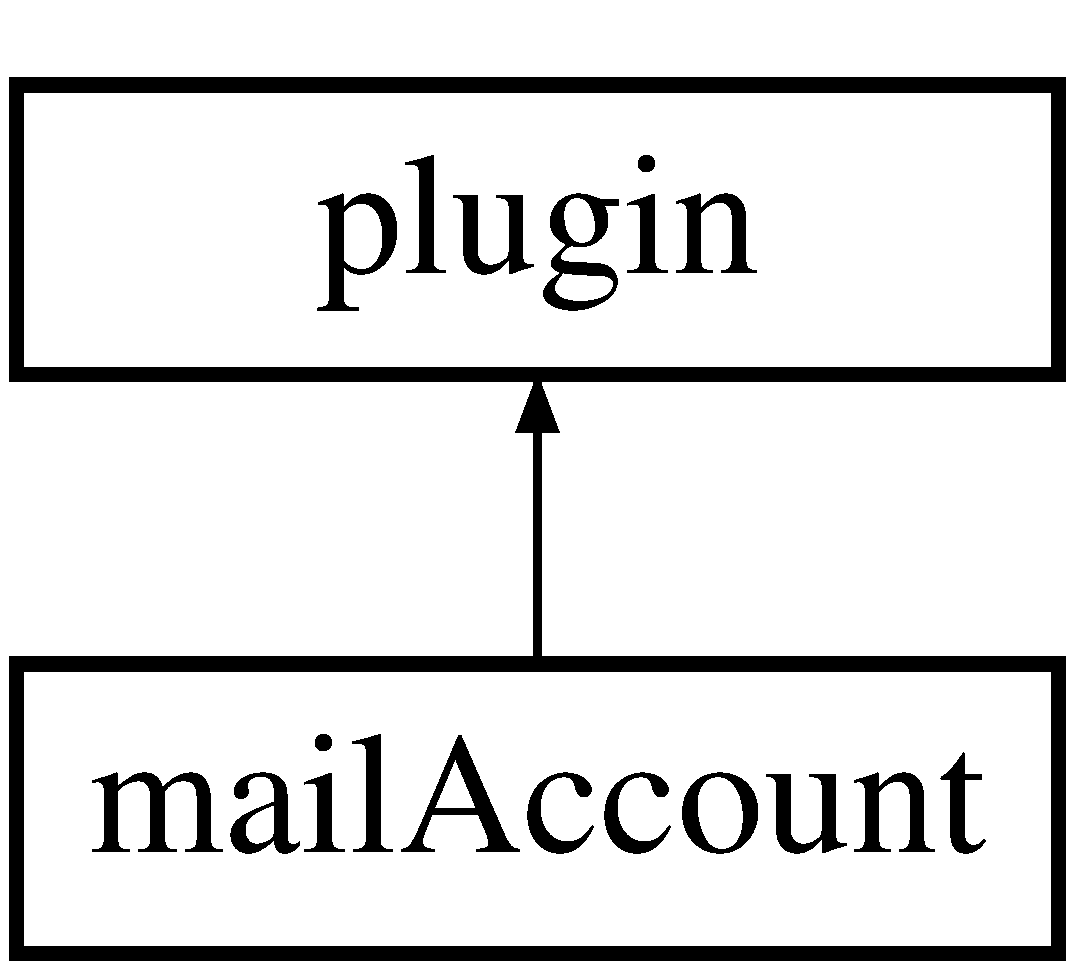
\includegraphics[height=2cm]{classmailAccount}
\end{center}
\end{figure}
\subsection*{Public Member Functions}
\begin{CompactItemize}
\item 
{\bf mail\-Account} (\${\bf dn}=NULL, \$shared\_\-folder=FALSE)\label{classmailAccount_a0}

\item 
{\bf get\-Imap\-Attributes} ()\label{classmailAccount_a1}

\item 
{\bf set\-Imap\-Attributes} ()\label{classmailAccount_a2}

\item 
{\bf set\-Sieve\-Attributes} ()\label{classmailAccount_a3}

\item 
{\bf execute} ()
\begin{CompactList}\small\item\em execute plugin \item\end{CompactList}\item 
{\bf remove\_\-from\_\-parent} ()\label{classmailAccount_a5}

\item 
{\bf save\_\-object} ()\label{classmailAccount_a6}

\item 
{\bf save} ()\label{classmailAccount_a7}

\item 
{\bf check} ()\label{classmailAccount_a8}

\item 
{\bf adapt\_\-from\_\-template} (\${\bf dn})\label{classmailAccount_a9}

\item 
{\bf add\-Forwarder} (\$address)\label{classmailAccount_a10}

\item 
{\bf del\-Forwarder} (\$addresses)\label{classmailAccount_a11}

\item 
{\bf add\-Alternate} (\$address)\label{classmailAccount_a12}

\item 
{\bf del\-Alternate} (\$addresses)\label{classmailAccount_a13}

\end{CompactItemize}
\subsection*{Public Attributes}
\begin{CompactItemize}
\item 
{\bf mail} = \char`\"{}\char`\"{}\label{classmailAccount_o0}

\item 
{\bf gosa\-Mail\-Alternate\-Address} = array()\label{classmailAccount_o1}

\item 
{\bf gosa\-Mail\-Forwarding\-Address} = array()\label{classmailAccount_o2}

\item 
{\bf gosa\-Mail\-Delivery\-Mode} = \char`\"{}[L ]\char`\"{}\label{classmailAccount_o3}

\item 
{\bf gosa\-Mail\-Server} = \char`\"{}\char`\"{}\label{classmailAccount_o4}

\item 
{\bf gosa\-Mail\-Quota} = \char`\"{}\char`\"{}\label{classmailAccount_o5}

\item 
{\bf gosa\-Mail\-Max\-Size} = \char`\"{}\char`\"{}\label{classmailAccount_o6}

\item 
{\bf gosa\-Vacation\-Message} = \char`\"{}\char`\"{}\label{classmailAccount_o7}

\item 
{\bf gosa\-Spam\-Sort\-Level} = \char`\"{}\char`\"{}\label{classmailAccount_o8}

\item 
{\bf gosa\-Spam\-Mailbox} = \char`\"{}\char`\"{}\label{classmailAccount_o9}

\item 
{\bf quota\-Usage} = 0\label{classmailAccount_o10}

\item 
{\bf forward\_\-dialog} = FALSE\label{classmailAccount_o11}

\item 
{\bf folder\_\-prefix} = \char`\"{}\char`\"{}\label{classmailAccount_o12}

\item 
{\bf mailbox\-List} = array()\label{classmailAccount_o13}

\item 
{\bf default\_\-permissions} = \char`\"{}none\char`\"{}\label{classmailAccount_o14}

\item 
{\bf member\_\-permissions} = \char`\"{}post\char`\"{}\label{classmailAccount_o15}

\item 
{\bf members} = array()\label{classmailAccount_o16}

\item 
{\bf admins} = array()\label{classmailAccount_o17}

\item 
{\bf perms}
\item 
{\bf attributes}
\item 
{\bf objectclasses} = array(\char`\"{}gosa\-Mail\-Account\char`\"{})\label{classmailAccount_o20}

\end{CompactItemize}


\subsection{Detailed Description}
mail plugin 

\begin{Desc}
\item[Author:]Cajus Pollmeier $<${\tt pollmeier@gonicus.de}$>$ \end{Desc}
\begin{Desc}
\item[Version:]2.00 \end{Desc}
\begin{Desc}
\item[Date:]24.07.2003\end{Desc}
This class provides the functionality to read and write all attributes relevant for gosa\-Mail\-Accounts from/to the LDAP. It does syntax checking and displays the formulars required. 



\subsection{Member Function Documentation}
\index{mailAccount@{mail\-Account}!execute@{execute}}
\index{execute@{execute}!mailAccount@{mail\-Account}}
\subsubsection{\setlength{\rightskip}{0pt plus 5cm}mail\-Account::execute ()}\label{classmailAccount_a4}


execute plugin 

Generates the html output for this node 

Reimplemented from {\bf plugin} {\rm (p.\,\pageref{classplugin_a1})}.

\subsection{Member Data Documentation}
\index{mailAccount@{mail\-Account}!attributes@{attributes}}
\index{attributes@{attributes}!mailAccount@{mail\-Account}}
\subsubsection{\setlength{\rightskip}{0pt plus 5cm}mail\-Account::attributes}\label{classmailAccount_o19}


{\bf Initial value:}

\footnotesize\begin{verbatim} array("mail", "gosaMailServer", "gosaMailQuota", "gosaMailMaxSize",
                        "gosaMailDeliveryMode", "gosaSpamSortLevel", "gosaSpamMailbox",
                        "gosaVacationMessage", "uid")
\end{verbatim}\normalsize 


Reimplemented from {\bf plugin} {\rm (p.\,\pageref{classplugin})}.\index{mailAccount@{mail\-Account}!perms@{perms}}
\index{perms@{perms}!mailAccount@{mail\-Account}}
\subsubsection{\setlength{\rightskip}{0pt plus 5cm}mail\-Account::perms}\label{classmailAccount_o18}


{\bf Initial value:}

\footnotesize\begin{verbatim} array( "lrs" => "read", "lrsp" => "post", "lrsip" => "append",
                        "lrswipcd" => "write", "lrswipcda" => "all" )
\end{verbatim}\normalsize 


The documentation for this class was generated from the following file:\begin{CompactItemize}
\item 
class\_\-mail\-Account.inc\end{CompactItemize}
